\documentclass[11pt]{article}
\usepackage[margin=1.15in]{geometry}
\usepackage{amsmath,amssymb}
\usepackage{booktabs}
\usepackage{graphicx}
\usepackage{natbib}
\usepackage[hidelinks]{hyperref}
% run-in headings italic, not bold (house style)
\makeatletter
\renewcommand\paragraph{\@startsection{paragraph}{4}{\z@}%
  {3.25ex \@plus1ex \@minus.2ex}{-1em}%
  {\normalfont\normalsize\itshape}}
\makeatother
\emergencystretch=1.5em

\title{Covariance-Method Claims Are Ensemble-Relative:\\
Named Measures and an Audit Program}
\author{Peter Cotton\thanks{\texttt{peter.cotton@microprediction.com}. The
ensemble library is \texttt{pip install randomcov}; the seeded scripts behind
every number here live beside this paper at
\texttt{github.com/microprediction/randomcov}.}}
\date{August 2026}

\begin{document}
\maketitle

\begin{abstract}
A claim about the behavior of a covariance or correlation method is a
claim about a distribution over matrices, and the distribution is rarely
stated. We measure how much that omission matters. Across fifteen named,
seeded ensembles at identical dimension and sample size, the
Ledoit--Wolf shrinkage intensity ranges from $0.07$ to $0.86$, and eleven
audited claims from eleven fields flip verdict as the ensemble changes,
for stated structural reasons. The \texttt{randomcov} library names the
measures and seeds the draws, so any claim can be re-run under all
fifteen; the results assemble into a matrix of claims against measures,
and a joint leaderboard of scikit-learn and \texttt{precise} estimators
has five different winners. The pattern survives scale: six of seven
claims re-run from $n=30$ to $n=3000$ keep their verdict, and the
seventh, hierarchical risk parity, flips under its own home-turf
ensemble as dimension grows. Eleven audits are completed here; a docket
from astronomy, genomics, neuroscience, and chemometrics, including
ensemble-invariant null controls, is assembled for the rest.
\end{abstract}

\section{The unstated measure}

Empirical claims about covariance methods have the form ``estimator $A$
beats estimator $B$,'' ``the shrinkage intensity is typically moderate,''
``the factorization recovers structure,'' with performance averaged over
random test matrices. That average is taken with respect to some
generating law, and in practice the law is inherited from convenience and
from the field. Finance validates on equity panels;
econophysics on the same panels with random-matrix nulls; geostatistics
on smooth kernels; psychometrics on low-rank factor models; graphical
modeling on sparse precisions; cosmology on mock catalogs of ordered
correlation-function bins.

Different laws produce matrices with different spectra, different
locality, and different factor content. A verdict certified under one law
therefore carries no warrant under another. What
the measurements below show is that this omission is not a mere
technicality.

\section{Precedents}

We are hardly the first to notice that method comparisons inherit their
verdicts from the simulation design; this is established already in
several literatures. \citet{morris2019} require simulation studies to
declare the data-generating mechanism as a design choice of equal rank
with the estimand. \citet{boulesteix2013} trace the over-optimism of
self-reported comparisons to test beds chosen by the method's own
authors. \citet{niessl2022} re-analyze one benchmark under hundreds of
design and analysis options and find that almost any method can reach
almost any rank. \citet{hooker1995} made the complaint for heuristics;
\citet{wolpert1997} give the limit statement, that averaged over all
objectives all optimizers tie.

The correlation-matrix version also has precedent.
\citet{joe2006} and \citet{lkj2009} supply the standard samplers.
\citet{hardin2013} argue that the habitual generators produce unrealistic
matrices and bias the evaluation of statistical techniques, and propose a
better one. \citet{marti2020} learns a generator from financial
correlation matrices and reports, in accompanying experiments, that the
HRP advantage fades on matrices without hierarchical
structure, a result restated in \citet{marti2021}.
\citet{papenbrock2021} evolve synthetic correlations to ask which
correlation structures favor which allocator. \citet{alvarez2014} document the Bayesian
mirror image: an inverse-Wishart prior biases the posterior variance upward
and the correlation toward zero when the true variance is small relative to
the prior mean, and the bias persists as the sample grows.

What the present paper adds is the instrument and the audits: a fixed
battery of fifteen named, seeded, public measures; the re-execution of
eleven published claims from eleven fields under all of them; the
claims-by-measures matrix as the reporting format; and provably invariant
theorems run as null controls.

\section{Fifteen named ensembles}

\texttt{randomcov} generates correlation matrices under fifteen named,
seeded measures, and the names describe the constructions:
\texttt{lkj}, \texttt{onion}, \texttt{vine} (elliptope samplers;
\citealp{joe2006,lkj2009}); \texttt{wishart}, \texttt{spectrum}
(prescribed spectral laws); \texttt{factor}, \texttt{hierarchical},
\texttt{block\_equicorr} (low-rank and clustered structure); \texttt{ar1},
\texttt{kernel} (banded and locality-driven fields);
\texttt{sparse\_precision} (graphical-model structure);
\texttt{archakov\_hansen} (log-matrix parameterization;
\citealp{archakov2021});
\texttt{residuals}, \texttt{walk}, \texttt{animals} (empirical-flavored
and trajectory ensembles).

Variance vectors are drawn separately, so correlation structure and scale
can be crossed independently. Every generator accepts an explicit seed,
and every number in this paper descends from one; there is no number
here we cannot regenerate. The scripts sit beside the paper.

Three of the fifteen are constructions of one measure. \texttt{lkj},
\texttt{onion} and \texttt{vine} each sample LKJ($\eta$) by a different
route, and they agree: across the eleven audits below their verdicts match
to within sampling noise, and they rank seventeen estimators in
near-identical order. That agreement is a check on the instrument. When
three routes to one law return one answer, a disagreement between laws is
a property of the laws.

\section{Two demonstrations}\label{sec:lw-demo}

We begin with the Ledoit--Wolf shrinkage estimator because it is used
across so many applications and because its diagnostic is easy to read:
the intensity says how far the sample covariance should be pulled toward
a target. Fix $n=30$ variables, each observed $T=60$ times, and draw
twenty panels per ensemble. This is not close to the $n=T$ boundary, and
Table~\ref{tab:lw} shows the variation anyway.

\begin{table}[t]
\centering\small
\begin{tabular}{lcc}
\toprule
ensemble & intensity & sd \\
\midrule
residuals & $0.072$ & $(0.019)$ \\
animals & $0.072$ & $(0.013)$ \\
factor & $0.101$ & $(0.038)$ \\
archakov\_hansen & $0.120$ & $(0.022)$ \\
kernel & $0.132$ & $(0.082)$ \\
walk & $0.199$ & $(0.038)$ \\
block\_equicorr & $0.247$ & $(0.096)$ \\
vine & $0.355$ & $(0.022)$ \\
lkj & $0.363$ & $(0.024)$ \\
onion & $0.363$ & $(0.030)$ \\
hierarchical & $0.369$ & $(0.070)$ \\
ar1 & $0.469$ & $(0.226)$ \\
wishart & $0.506$ & $(0.032)$ \\
spectrum & $0.532$ & $(0.058)$ \\
sparse\_precision & $0.862$ & $(0.066)$ \\
\bottomrule
\end{tabular}
\caption{Ledoit--Wolf shrinkage intensity by ensemble at $n=30$, $T=60$:
mean and standard deviation over twenty seeded draws.}\label{tab:lw}
\end{table}

The intensity spans $0.072$ to $0.862$ at identical $(n,T)$. A paper
reporting ``typical'' shrinkage from one generator is reporting a property
of its generator. The ordering is interpretable: strong low-rank structure
(\texttt{animals}, \texttt{residuals}, \texttt{factor}) wants little
shrinkage, and near-unstructured draws (\texttt{wishart},
\texttt{sparse\_precision}) want a great deal. The within-ensemble
standard deviation is informative too; \texttt{ar1} spans $0.23$ across
its own parameter draws.

The second demonstration is software of our own. A deterministic
algorithm for multinomial probit choice probabilities (the
\texttt{winning} package; paper in that repository) reports median
absolute error by ensemble after fitting a structured covariance grammar.
For twelve of the fifteen measures the error is $1$--$4\times10^{-5}$; for
the dense, strongly correlated ensembles it is $1$--$4\times10^{-4}$, and
under \texttt{kernel} fields $4\times10^{-3}$, because the fit does not
yet admit the band-diagonal structure a kernel covariance calls for. A
validation run on any single ensemble would have reported either
``essentially exact'' or ``inadequate,'' both correctly, for the same
method. That experience was much of the motivation for writing the
generator library.

\section{Eleven audits, eleven fields}

The same brittleness might apply more broadly, and where it does there
is room to improve existing tools. The method is short. We take a
published claim, re-run its demonstration under every generator in the
library, and report the verdict.

We audit one claim from each of eleven fields: seven about estimators and
constructions (Table~\ref{tab:audits}) and four about inference and
dimensionality (Table~\ref{tab:rates}). Figure~\ref{fig:matrix} assembles
the results into a single matrix and outlines each claim's \emph{home
turf}, the correlation structure it was demonstrated on or intended for,
as best we can tell. All runs
use $n=30$ with twenty replications unless stated. Sampled panels use
$T=60$ except where the claim's own regime dictates otherwise.

\paragraph{Finance.} We start here because it is the field we know best.
\citet{lopezdeprado2016} reports that hierarchical
risk parity delivers lower out-of-sample variance than a long-only,
fully-invested quadratic minimum-variance optimizer, and names estimation
error in the inverse as the culprit. We
build both portfolios from the same sample covariance and score the true
variance $w^{\top}\Sigma w$ under the generating covariance. Column~1 of
Table~\ref{tab:audits} gives the median ratio of HRP to long-only minimum
variance.

HRP wins on every draw under \texttt{sparse\_precision} and
splits draws roughly evenly under \texttt{ar1} and \texttt{hierarchical},
the ensembles whose dependency structure the bisection tree can match; it
loses by an order of magnitude or more under \texttt{animals},
\texttt{factor}, and \texttt{archakov\_hansen}, where the true matrix
rewards positions a long-only tree cannot take. Against unconstrained
minimum variance the losses grow by many more orders of magnitude: the
median ratio is $\sim\!10^{8.7}$ under \texttt{walk} and $\sim\!10^{11.2}$
under \texttt{residuals}, because near-singular ensembles admit
near-perfect hedges that only signed weights can reach. Both of those
ensembles reach the positive-semidefinite floor, and the exponent scales
inversely with the clip, falling a decade for every decade the clip
loosens. The ensemble sets the direction of the result and the floor sets
its size.

\paragraph{Econophysics.} \citet{laloux1999} find the bulk of the sample correlation spectrum
indistinguishable from Marchenko--Pastur noise. The cleaning recipe that
follows, flattening every eigenvalue below the edge $(1+\sqrt{n/T})^{2}$
and reporting the result, is \citet{laloux2000}. Column~2 gives the
Frobenius-loss ratio of clipped to raw sample correlation. The cleaning is
excellent under \texttt{sparse\_precision} ($0.30$) and
\texttt{hierarchical} ($0.76$), and it damages the estimate under eleven
of fifteen ensembles, worst at $1.43$--$1.77$ under \texttt{animals},
\texttt{kernel}, \texttt{archakov\_hansen}, and \texttt{residuals}.

The mechanism is not quite the textbook one. \texttt{hierarchical} does
carry a spike over a bulk. \texttt{sparse\_precision} carries none, with a
largest true eigenvalue of $1.43$ against an edge of $2.91$, and clipping
wins there because the sub-edge spectrum is nearly flat already, so
flattening it costs almost nothing. Under the four worst ensembles the
sub-edge mass is dispersed, and flattening erases genuine structure as
noise. What predicts the verdict is the dispersion of the true spectrum
below the edge. The recipe presumes that signal means spikes, and locality
puts signal in the bulk.

\paragraph{Geostatistics.} The screening effect of \citet{stein2002} says
that a few nearest neighbors, here the most correlated, nearly attain the
full kriging variance. This is a population property, so no sampling is
involved. Column~3 reports the median ratio of conditional variance given
the best five predictors to conditional variance given all $n-1$.
Screening holds to within a few per cent under \texttt{ar1} (Markov,
ratio $1.00$), \texttt{hierarchical}, and \texttt{block\_equicorr}. It also reads
$1.00$ under \texttt{sparse\_precision}, but vacuously: conditioning on all
$n-1$ neighbors removes only about four per cent of the variance there, so
there is nothing for five neighbors to miss.

Screening fails several-fold under the elliptope samplers \texttt{lkj},
\texttt{onion} and \texttt{vine}, and under \texttt{kernel} itself ($5.7$).
Every \texttt{kernel} draw is squared-exponential, whose spectral density
decays faster than any algebraic rate and so falls outside Stein's
conditions; interpolation is nearly deterministic from all sites but not
from five. The failure tracks the drawn length scale almost perfectly
(correlation $0.98$ between length scale and log ratio), and a Mat\'ern-3/2
field on the identical point clouds gives $1.04$ instead. That is Stein's
own caveat, that screening depends on smoothness, reproduced as a
contrast.

\paragraph{Psychometrics.} Parallel analysis \citep{horn1965} retains the components whose sample
eigenvalues exceed those of independent data of the same shape. Horn
compared against the mean null eigenvalue; we use the now-standard
95th-percentile form of \citet{glorfeld1995}. It is the standard answer
to ``how many factors?'' Column~4 gives the mean retained count: $1.8$
under \texttt{sparse\_precision} to $7.3$ under \texttt{onion} at
identical $(n,T)$, more than a fourfold spread for what is supposed to be
an objective count.

The same sweep scores the eigenvalue-greater-than-one rule of \citet{kaiser1960} against the population count of
eigenvalues above one. Kaiser over-extracts under \texttt{factor} ($5.7$
retained against $3.0$ true), under-extracts under \texttt{wishart}
($11.2$ against $13.1$), and disagrees with parallel analysis by a factor
that is itself ensemble-dependent: $1.4$ under \texttt{residuals}, $7$
under \texttt{sparse\_precision}. The number of factors a study reports is
therefore, in part, a property of the generating measure its data happen
to resemble.

\paragraph{Data assimilation.} Ensemble Kalman filtering runs with far
fewer members than state variables, and the standard remedy is covariance
localization: taper the sample covariance entrywise with a Gaspari--Cohn
function \citep{gaspari1999} of inter-variable distance
\citep{houtekamer2001,hamill2001}. \citet{paz2015} apply the closely
related covariance tapering of \citet{kaufman2008} to correlation-function
bins, with a Wendland taper and a two-taper precision estimator. The two
share the assumption this audit tests, that the taper coordinate carries
the truth's locality, so the audit applies to both fields. With $N=20$
members for $n=30$ variables and a taper of index distance with
half-radius $6$, column~5 reports the Frobenius-loss ratio of tapered to
raw.

The split is interpretable. Localization helps wherever the estimate is
noisy and the truth carries no long-range structure in taper coordinates,
including under the dense elliptope samplers, where variance reduction
beats the bias. It hurts under \texttt{factor}, \texttt{animals}, and
\texttt{residuals} ($1.66$--$1.84$), whose common factors are long-range
by construction. It also hurts under \texttt{kernel} ($1.46$), the one
ensemble that is local by construction,
because kernel locality lives in a latent two-dimensional point cloud
rather than in index order. Localization requires locality in the
coordinates the taper can see.

\paragraph{Signal processing.} Diagonal loading is the standard repair
for the sample-covariance MVDR beamformer: \citet{cox1987} derive it from a
constraint on white-noise array gain, against sensor and steering
perturbations, and \citet{carlson1988} tie it to covariance estimation error
in the snapshot-limited regime. With $T=40$ snapshots, a
random unit steering vector, the distortionless constraint, and loading
$\delta=0.1\,\mathrm{tr}(\hat\Sigma)/n$, column~6 reports the median
ratio of true output power, loaded over unloaded. The picture is mixed. Loading roughly halves the output power under six
of the fifteen ensembles, which is the win it is sold as, and multiplies
it under \texttt{archakov\_hansen} ($20.5$), \texttt{animals} ($33$),
\texttt{kernel} ($136$), \texttt{residuals} ($10^{7.7}$), and
\texttt{walk} ($10^{7.9}$). The mechanism
is the hedge from the finance audit seen from the other side: under
near-singular ensembles the beamformer's null-steering lives in the
smallest eigenvalues, which is exactly what loading erases.

\paragraph{Graphical modeling.} The graphical lasso of \citet{friedman2008} made the sparsity prior on the
precision matrix cheap enough to be routine. Their own claim was speed;
the field attached to it the promise that the prior improves estimation. That promise underwrites partial-correlation connectomes
\citep{smith2011} and sparse cosmological precision matrices
\citep{padmanabhan2016}. Column~7
reports the Frobenius loss of the cross-validated glasso precision
against the true precision, relative to inverting a Ledoit--Wolf
shrinkage estimate of the kind \citet{schafer2005} recommend for gene
networks.

The sparsity prior wins where precisions are sparse or banded, at $0.69$
under \texttt{ar1}, $0.68$ under \texttt{hierarchical}, and $0.63$ under
\texttt{sparse\_precision}. It ties across the dense elliptope middle. It loses
under \texttt{factor} ($1.09$), and under \texttt{residuals} it ties at
$1.00$ while winning on none of the twenty draws. Dense low-rank structure
is the worst case for sparsity.

\begin{table}[t]
\centering\footnotesize
\setlength{\tabcolsep}{4.5pt}
\begin{tabular}{lccccccc}
\toprule
 & HRP/MV & clip/raw & near/full & PA count & taper/raw & load/raw & gl/LW \\
ensemble & (fin.) & (econo.) & (geost.) & (psych.) & (assim.) & (sig.\
proc.) & (graph.) \\
\midrule
animals & $8.38$ & $1.43$ & $5.53$ & $3.3$ & $1.66$ & $32.8$ & $1.00$ \\
ar1 & $0.98$ & $1.20$ & $1.00$ & $4.5$ & $0.53$ & $0.48$ & $0.69$ \\
archakov\_hansen & $71.8$ & $1.47$ & $131$ & $4.7$ & $1.41$ & $20.5$ & $1.00$ \\
block\_equicorr & $1.09$ & $1.00$ & $1.04$ & $3.0$ & $1.00$ & $0.55$ & $0.78$ \\
factor & $12.3$ & $1.38$ & $1.06$ & $2.2$ & $1.69$ & $0.94$ & $1.09$ \\
hierarchical & $1.00$ & $0.76$ & $1.02$ & $2.3$ & $0.82$ & $0.45$ & $0.68$ \\
kernel & $1.51$ & $1.46$ & $5.69$ & $4.1$ & $1.46$ & $136$ & $1.00$ \\
lkj & $2.67$ & $1.29$ & $10.6$ & $7.3$ & $0.79$ & $2.26$ & $0.99$ \\
onion & $2.83$ & $1.29$ & $9.04$ & $7.3$ & $0.78$ & $3.29$ & $1.00$ \\
residuals & $2.75$ & $1.77$ & $\sim\!10^{8.3}$ & $4.0$ & $1.84$ & $\sim\!10^{7.7}$ & $1.00$ \\
sparse\_precision & $0.76$ & $0.30$ & $1.00$ & $1.8$ & $0.50$ & $0.48$ & $0.63$ \\
spectrum & $1.11$ & $0.94$ & $1.32$ & $5.8$ & $0.66$ & $0.51$ & $0.99$ \\
vine & $2.68$ & $1.29$ & $11.9$ & $7.0$ & $0.81$ & $4.13$ & $1.00$ \\
walk & $1.23$ & $1.11$ & $\sim\!10^{8.7}$ & $3.7$ & $1.14$ & $\sim\!10^{7.9}$ & $1.00$ \\
wishart & $1.19$ & $1.04$ & $1.50$ & $6.5$ & $0.66$ & $0.51$ & $0.95$ \\
\bottomrule
\end{tabular}
\caption{Seven audited claims about estimators and constructions; all
entries are medians over twenty seeded draws. Column 1: out-of-sample
true-variance ratio, HRP over long-only minimum variance (below one: HRP
wins). Column 2: Frobenius-loss ratio, Marchenko--Pastur-clipped over raw
sample correlation (below one: cleaning helps). Column 3: population
conditional-variance ratio, five best predictors over all (near one:
screening holds). Column 4: mean components retained by parallel
analysis. Column 5: Frobenius-loss ratio, Gaspari--Cohn-tapered over raw
sample covariance at $N=20$ members (below one: localization helps).
Column 6: true beamformer output power, diagonally loaded over unloaded
at $T=40$ snapshots (below one: loading helps). Column 7:
precision-matrix Frobenius-loss ratio, cross-validated graphical lasso
over inverted Ledoit--Wolf (below one: the sparsity prior wins). Each
column's verdict flips across rows. \texttt{walk} and \texttt{residuals}
are rank-deficient by construction and reach the positive-semidefinite
floor, so their entries in the two inverse-sensitive columns (3 and 6) are
set by that floor: the exponents scale inversely with the clip and would
move decade for decade under a looser one. They establish failure and
nothing more precise than that.}\label{tab:audits}
\end{table}

We also performed a smaller companion study. With oracle shrinkage intensities, the
constant-correlation target of \citet{ledoit2004honey} beats the
scaled-identity target of \citet{ledoit2004} on every draw under \texttt{sparse\_precision}
(median loss ratio $0.62$) and wins on only three of twenty draws under
\texttt{factor}, where the two targets are otherwise indistinguishable at
a median ratio of $1.00$. Even the choice between two targets from the same
authors is ensemble-relative.

The remaining four claims concern hypothesis tests, rates and counts
(Table~\ref{tab:rates}).

\paragraph{Evolutionary biology.} \citet{cheverud1996} declares two genetic
covariance matrices similar when their mean response-vector correlation
under common random selection gradients exceeds the null for independent
random vectors. We apply the test to independent pairs drawn from the
same ensemble. This is a population property with no sampling noise, so a
sound test should declare similarity about $5\%$ of the time. It is at or below nominal
under \texttt{factor} and \texttt{archakov\_hansen} ($0\%$) and
\texttt{animals} ($10\%$), and declares independent matrices similar
$100\%$ of the time under eleven of the fifteen ensembles.
\citet{cheverud2007} concede as much in passing: in practice the null of
no shared structure ``is nearly always rejected.''

Under \texttt{sparse\_precision} the mean skewers correlation between
independent matrices is $0.97$, because near-diagonal matrices respond to
any skewer with the skewer itself. \citet{rohlf2017} raises this objection
in general terms.

\paragraph{Climatology.} \citet{north1982} give a rule of thumb: when an eigenvalue's sampling error
$\lambda\sqrt{2/T}$ is comparable to the spacing to a neighbor, the sampling
error in the associated EOF is comparable to the neighboring EOF. They draw the converse as a first-order corollary, that a stand-out
eigenvalue has small EOF sampling error, and say plainly that the rule
offers no guidance on where to truncate. It is the corollary we score.

We score the false-reassurance rate: among draws the rule declares
separated, how often the leading sample eigenvector is mostly wrong
(squared alignment with the truth below one half). The rate is $0\%$ under six
ensembles, $57\%$ under \texttt{wishart}, and $100\%$ under
\texttt{sparse\_precision}, which declares separation on only $12\%$ of
draws but is always wrong when it does. The rule is a first-order
perturbation statement: excellent for spiked spectra, and unreliable
exactly where spectra are quasi-degenerate.

\paragraph{Ecology.} \citet{guillot2013} report that the Mantel test
\citep{mantel1967} rejects independence between distance matrices at $25$--$55\%$ under
strong spatial autocorrelation, at nominal $5\%$. Our audit puts the
original claim and the critique on the same footing (two independent site
variables drawn with covariance $C$ with Euclidean distance matrices and $499$
label permutations). The realized type-I error is the nominal $5\%$ under
\texttt{onion} and \texttt{vine} (and $6\%$ under \texttt{lkj}), and
$38$--$43\%$ under \texttt{factor}, \texttt{kernel}, \texttt{animals},
and \texttt{residuals}. This reproduces the published inflation under
locality-and-factor structure and shows calibration under dense elliptope
measures. ``The Mantel test is broken'' and ``the Mantel test is fine''
are both correct reports, from different ensembles.

\paragraph{Quantitative genetics.} \citet{kirkpatrick2009} reports effective
dimension counts $n_D=\sum_i\lambda_i/\lambda_{\max}$ of roughly one to
two for published genetic covariance matrices, read as evolutionary
constraint. At the low precision typical of breeding designs, $T=15$
here, the estimated $n_D$ deflates the truth by an ensemble-dependent
factor. A true $n_D$ of $12.3$ under \texttt{sparse\_precision} is
reported as $5.2$ (ratio $0.42$), while \texttt{factor} and
\texttt{animals} are nearly undistorted ($0.90$, $0.89$) because their
truth is already low-dimensional. Across all fifteen ensembles the
estimate never exceeds $5.2$, whatever the truth. A low reported $n_D$ cannot by
itself distinguish low-dimensional biology from a noisy estimate of
diffuse structure.

\begin{table}[t]
\centering\small
\begin{tabular}{lcccc}
\toprule
 & skewers & North rule & Mantel & $n_D$ ratio \\
ensemble & false sim. & false reass. & type-I & est/true \\
\midrule
animals & $10\%$ & $0\%$ & $40\%$ & $0.89$ \\
ar1 & $100\%$ & $20\%$ & $13\%$ & $0.54$ \\
archakov\_hansen & $0\%$ & $9\%$ & $28\%$ & $0.78$ \\
block\_equicorr & $100\%$ & $0\%$ & $15\%$ & $0.77$ \\
factor & $0\%$ & $0\%$ & $38\%$ & $0.90$ \\
hierarchical & $100\%$ & $0\%$ & $6\%$ & $0.78$ \\
kernel & $100\%$ & $3\%$ & $39\%$ & $0.88$ \\
lkj & $100\%$ & $26\%$ & $6\%$ & $0.53$ \\
onion & $100\%$ & $33\%$ & $5\%$ & $0.57$ \\
residuals & $95\%$ & $0\%$ & $43\%$ & $0.92$ \\
sparse\_precision & $100\%$ & $100\%$ & $7\%$ & $0.42$ \\
spectrum & $100\%$ & $10\%$ & $9\%$ & $0.52$ \\
vine & $100\%$ & $33\%$ & $5\%$ & $0.55$ \\
walk & $100\%$ & $0\%$ & $8\%$ & $0.83$ \\
wishart & $100\%$ & $57\%$ & $7\%$ & $0.47$ \\
\bottomrule
\end{tabular}
\caption{Four audited claims about inference. Column 1: share of
independent matrix pairs that random skewers declares similar (sound:
$\approx 5\%$). Column 2: among draws North's rule declares separated,
share whose leading EOF is mostly wrong (squared alignment below
$\tfrac12$). Column 3: realized type-I error of the Mantel test at
nominal $5\%$. Column 4: estimated over true effective dimensions of a
covariance matrix at $T=15$ (undistorted: near one).}\label{tab:rates}
\end{table}

\begin{figure}[p]
\centering
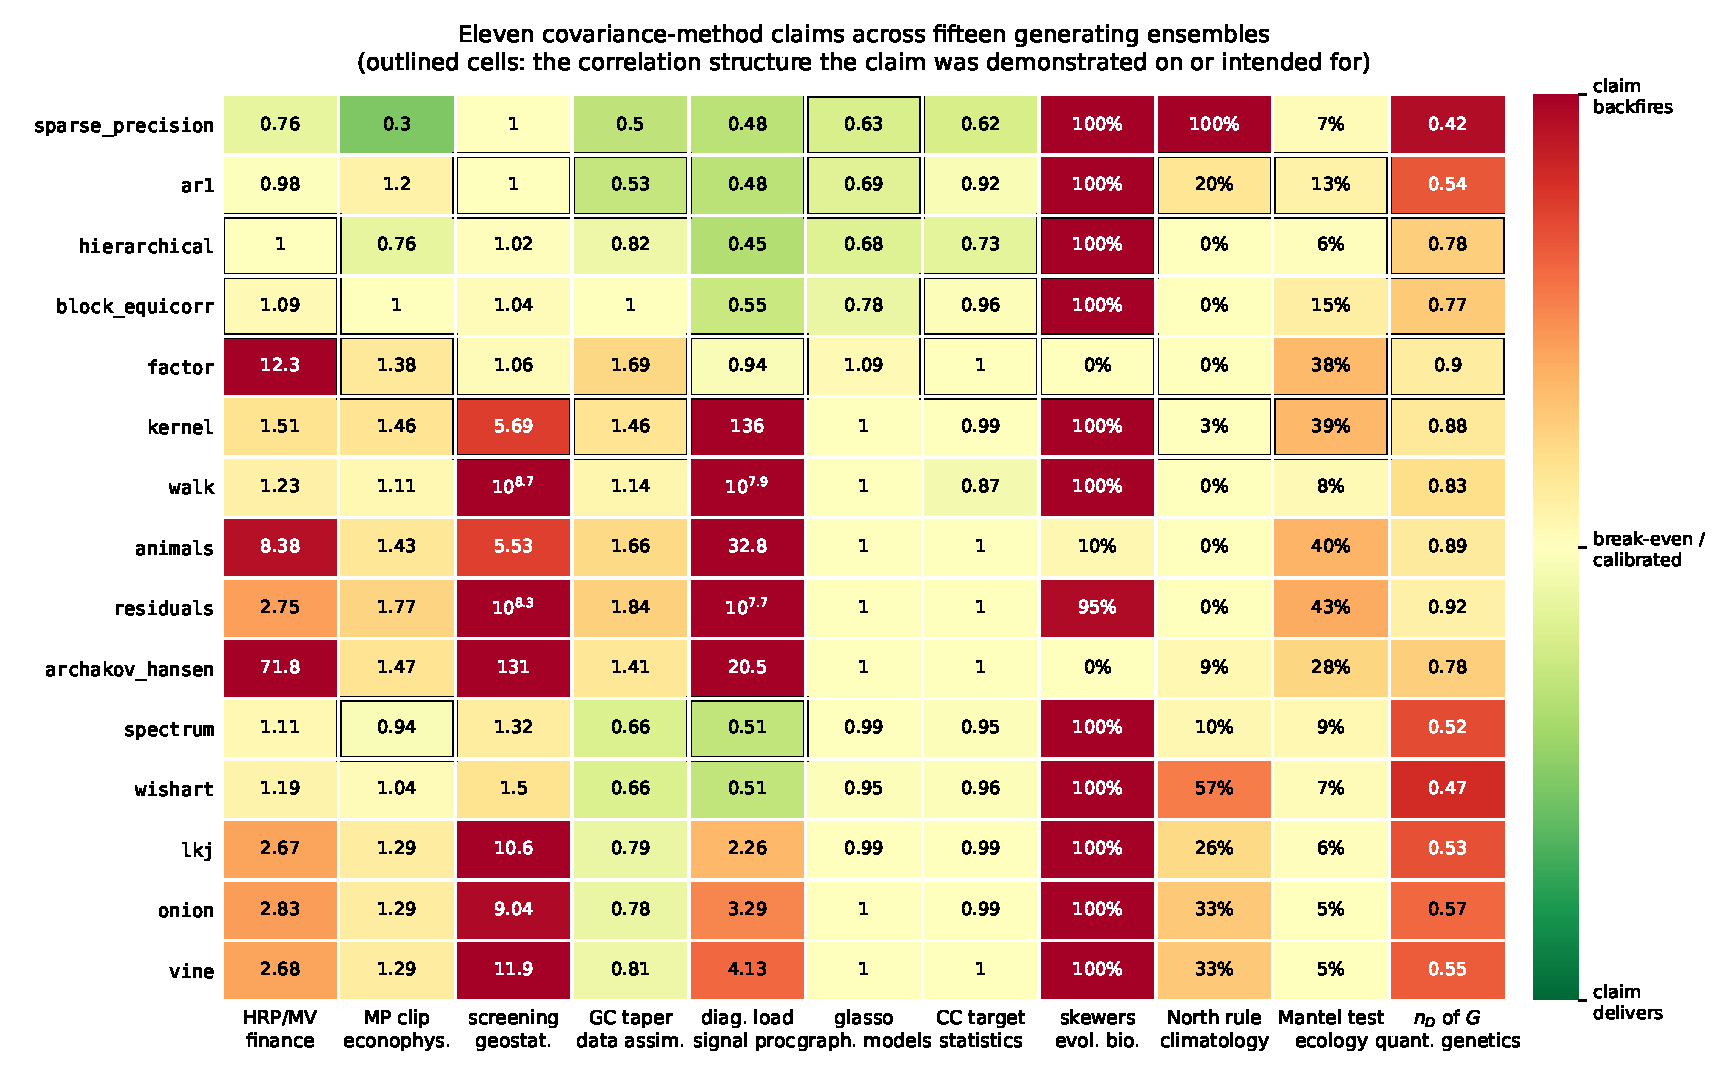
\includegraphics[width=\textwidth]{matrix.pdf}
\caption{The audit matrix: eleven claims (columns, with their fields)
against fifteen generating ensembles (rows, ordered roughly from
structured to dense). Green: the claim delivers under that measure.
Yellow: break-even or calibrated. Red: the claim backfires or the test is
broken. Cell entries are the medians and rates of
Tables~\ref{tab:audits} and~\ref{tab:rates}. Outlined cells mark each
claim's home turf, the correlation structure it was demonstrated on or
intended for.}\label{fig:matrix}
\end{figure}

\section{Do claims scale?}\label{sec:scale}

Every study above fixes $n=30$. A reasonable objection is that
ensemble-relativity is a small-panel artifact, that estimation noise
dominates at $n=30$ and would wash out with more assets. We re-run the
Ledoit--Wolf intensity demonstration of Section~\ref{sec:lw-demo} and five of the seven
Table~\ref{tab:audits} claims (finance, econophysics, data assimilation,
signal processing, and the graphical lasso, both the cross-validated
penalty and a fixed one) across a $5\times5$ grid, $n\in\{30, 100, 300,
1000, 3000\}$ crossed with $T/n\in\{0.5,1,2,4,8\}$, medians over
twenty-four seeded draws per cell (twelve at $n=1000$ and $n=3000$, for
cost). Figure~\ref{fig:scale} plots all thirty-five cells of every audit,
one line per ensemble. The two largest passes cost on the order of a
hundred worker-hours apiece.

The spread does not close. At $n=3000$, $T/n=1$, the Ledoit--Wolf
intensity still ranges from $0.002$ (\texttt{factor}) to $0.780$
(\texttt{sparse\_precision}), a wider ratio than the $0.157$--$0.720$
spread we saw at $n=30$. Marchenko--Pastur clipping helps \texttt{sparse\_precision}
more as $n$ grows ($0.293\to0.148$ at $T/n=2$) and hurts \texttt{factor}
far more ($1.366\to9.432$); its verdict does not flip for a single
literature ensemble between $n=30$ and $n=3000$ at fixed $T/n=2$, and
neither does diagonal loading's, the graphical lasso's, or Gaspari--Cohn
tapering's.\footnote{The fixed-penalty graphical lasso records one
nominal flip, \texttt{lkj} from $1.004$ to $1.000$, indistinguishable
from a tie. The cross-validated graphical lasso is incomplete at
$n=1000$, roughly half its cells missing to per-cell timeouts, and
dropped entirely at $n=3000$, where a single fit runs into the hour.} So
for six of the seven claims re-run, a claim's ensemble-verdict at $n=30$
is a reliable predictor of its verdict at a hundred times the dimension.

The exception is hierarchical risk parity, but only under one of the two
ensembles that looked exceptional at $n=30$. At $n=30$, $T/n=2$, HRP
roughly breaks even against long-only minimum variance under
\texttt{ar1} and \texttt{hierarchical}, the two literature ensembles
whose structure the bisection tree is built to match (ratios $0.890$,
$0.962$, twenty-four draws). At $n=3000$, the twelve-draw grid median
moves to $1.259$ and $2.580$, both apparent losses. A targeted
replication at forty-eight draws confirms the \texttt{hierarchical} loss
(median $2.557$; every single draw favors minimum variance) and retracts the
\texttt{ar1} one: the forty-eight-draw median is $0.914$, $56\%$ of
draws still favor HRP, and the ratio ranges from $0.69$ to
$1.89$.\footnote{\texttt{hrp\_n3000\_replication.py}, beside this paper.
Reps~$0$--$11$ reuse the grid's own deterministic seeding; reps
$12$--$47$ extend it under the identical scheme.} The twelve-draw
estimate had landed on the high side of a noisy statistic. A rep count
that is fine for most cells is not automatically fine for all of them.

\texttt{sparse\_precision} remains an outright HRP win at every scale we
tested, and \texttt{ar1} remains close to a tie at every scale we
tested. Only \texttt{hierarchical} flips, and the cause is the
ensemble rather than the algorithm: its cluster correlation is a function
of absolute cluster size, so as $n$ grows the matrix thins toward plain
equicorrelation: its non-equicorrelation content falls fourfold from
$n=30$ to $n=3000$, and the share of pairs correlated above $0.2$ falls a
hundredfold. The structure HRP is built to exploit is gone by $n=3000$,
while the long-only quadratic
program keeps exact use of the full covariance regardless of $n$. A
home-turf verdict is not guaranteed to survive scale, and a low rep count
is not guaranteed to survive a check.

We checked the other close calls. At $n=3000$, $T/n=2$, three
literature ensembles sit within $2\%$ of the clip/raw$=1$ threshold on
the twelve-draw grid: \texttt{spectrum} ($0.996$), \texttt{kernel}
($1.017$), \texttt{archakov\_hansen} ($1.020$), closer calls than HRP's
\texttt{ar1} ever was. A forty-eight-draw check confirms all three
(medians $0.996$, $1.018$, $1.021$; no range wider than $[0.98,
1.06]$).\footnote{\texttt{clip\_n3000\_replication.py}, beside this
paper, same seeding scheme as the HRP check.} All three hold. The
difference from HRP is the statistic: a Frobenius-norm ratio has almost
no per-draw variance, while HRP's long-only optimizer does, so twelve
draws are trustworthy for one and not for the other. The fragility is a
property of the HRP audit's statistic.

Five of the fifteen ensembles turn numerically rank-deficient at the
largest dimensions tested and need a positive-semidefinite floor before
any audit runs: three package-native curiosities (\texttt{walk} on
$58\%$ of $n=3000$ panels, \texttt{residuals} on $33\%$,
\texttt{animals} on $17\%$) and two literature ensembles
(\texttt{archakov\_hansen} on $14\%$, \texttt{kernel} on $3\%$). The
floor is applied before scoring, so the numbers above already reflect
it; a reader citing an \texttt{archakov\_hansen} or \texttt{kernel}
verdict at $n=3000$ should know that a seventh to a thirtieth of its
draws needed rescue just to stay a valid correlation matrix.

\begin{figure}[p]
\centering
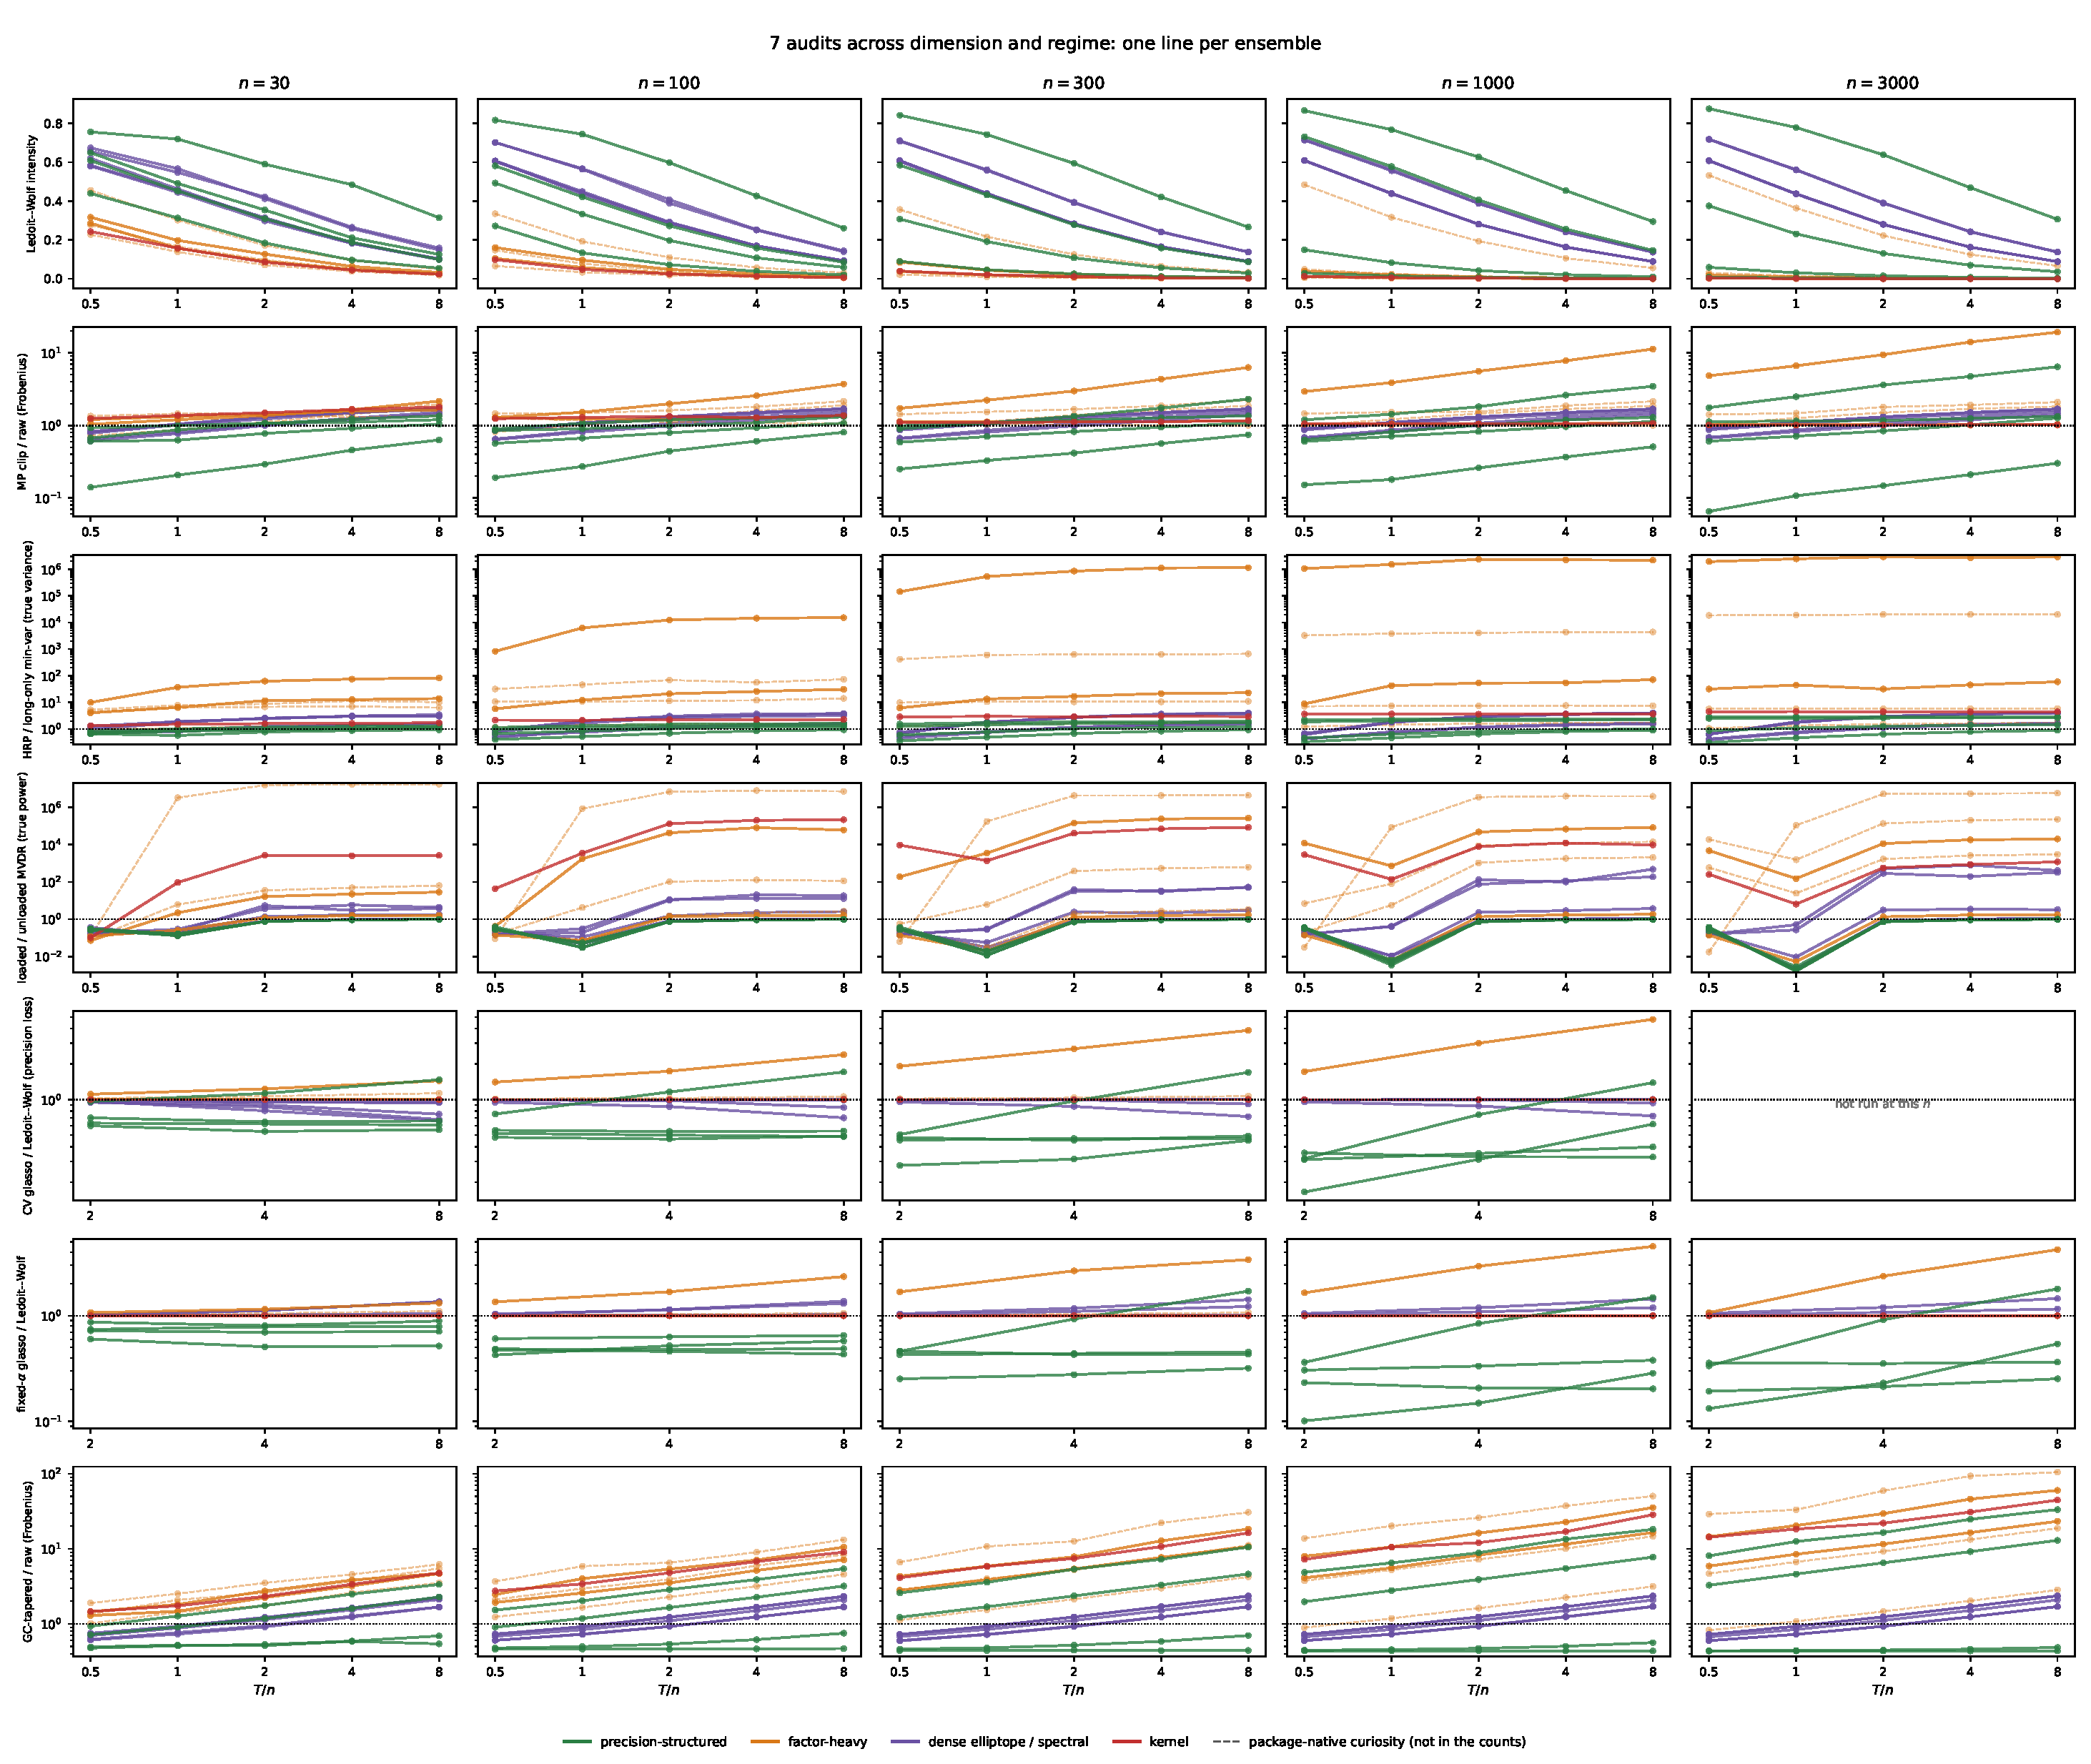
\includegraphics[width=\textwidth]{scale.pdf}
\caption{Seven audits (rows: Ledoit--Wolf intensity, MP clipping, HRP,
MVDR loading, cross-validated and fixed-penalty graphical lasso,
Gaspari--Cohn tapering) across five dimensions (columns, $n=30$ to
$3000$) and five regimes within each panel ($T/n=0.5$ to $8$), one line
per ensemble, colored by structural family; dashed lines are
package-native curiosities. Rows share a $y$-axis scale within each
audit so drift with $n$ is visible. Cross-validated glasso is not run at
$n=3000$.}\label{fig:scale}
\end{figure}

\section{One leaderboard per measure}

The audits test one claim at a time; the same harness can just as
easily rank whole libraries. We fit the six covariance estimators of scikit-learn and the
eleven batch-applicable estimators of \texttt{precise} to the same twenty
seeded panels per ensemble and rank them by median relative Frobenius
loss against the generating covariance (Figure~\ref{fig:ranking}). Five
estimators take first place somewhere: OAS on four ensembles, fixed
shrinkage and the graphical lasso on three each, Ledoit--Wolf on two, and,
perhaps surprisingly, the raw sample covariance on \texttt{animals},
\texttt{kernel} and \texttt{residuals}, three of the ensembles the
intensity table already marked as wanting almost no shrinkage. The
graphical lasso is first on the three precision-structured rows
(\texttt{sparse\_precision}, \texttt{ar1}, \texttt{hierarchical}) and
twelfth of seventeen under \texttt{animals}, \texttt{residuals}, and
\texttt{factor}, a large fall. The \texttt{precise} estimators are
built for time-varying covariance and pay for that design on static
panels, filling the lower ranks. A library default is a bet on a
measure, whether or not the author meant it that way.

\begin{figure}[p]
\centering
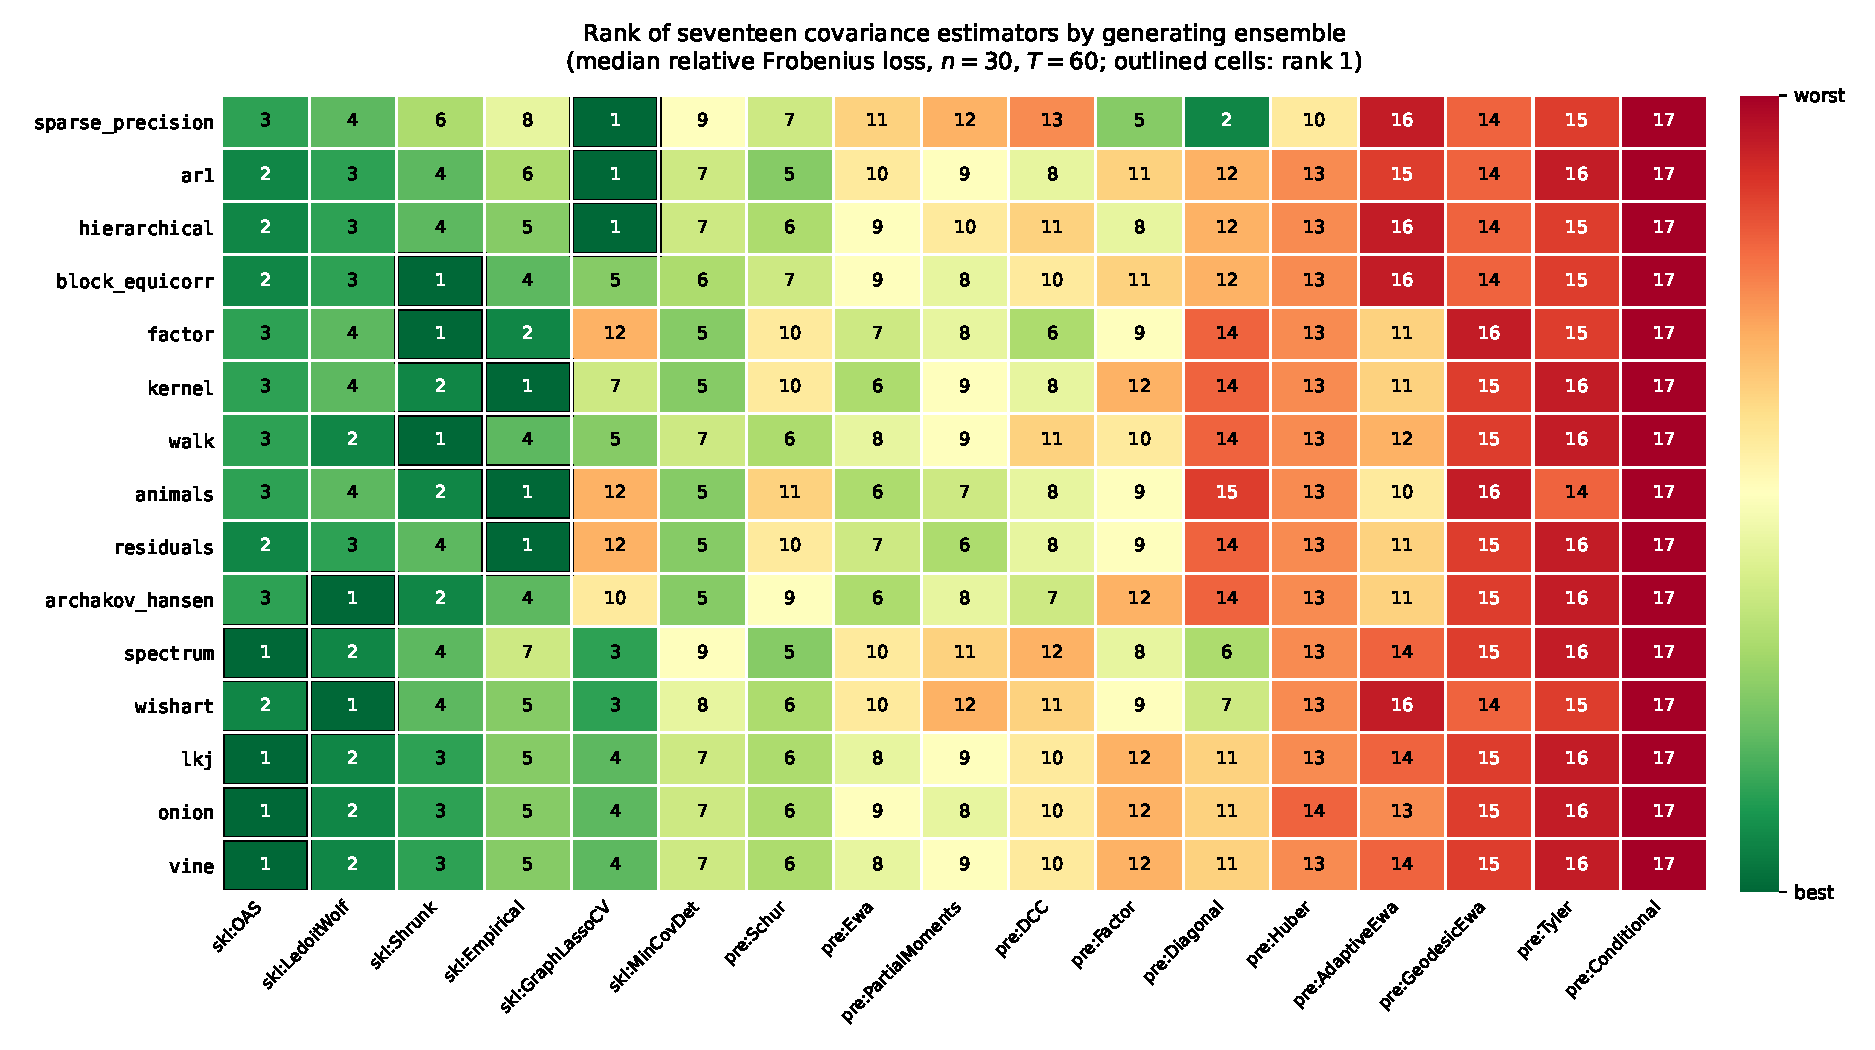
\includegraphics[width=\textwidth]{ranking.pdf}
\caption{The leaderboard matrix: seventeen covariance estimators, six
from scikit-learn and eleven from \texttt{precise}, ranked within each
generating ensemble by median relative Frobenius loss at $n=30$, $T=60$,
twenty seeded draws per ensemble. Rank-one cells are outlined; columns
are ordered by mean rank.}\label{fig:ranking}
\end{figure}

\section{Scope}

The audits measure the ensemble-sensitivity of a claim, often outside the
scope its authors gave it. Stein proved that screening depends on
smoothness; \citet{bickel2008} state the bandable class their banding
rates require; L\'opez de Prado demonstrated HRP on equity covariances and
said so; the data-assimilation literature has always tied localization to
physical distance.

The selection of claims is ours, and it leaned toward methods we knew to
be useful or hoped would be. A red cell in Figure~\ref{fig:matrix}
therefore says where a claim holds, and says nothing against the claim
where its authors placed it. Several audits run a method well outside the
regime it was built for, deliberately, because that is where second-hand
use puts it.

The battery is a choice too. Fifteen named measures are not a uniform
measure over correlation matrices, since no such thing exists, and they
are not exhaustive. Adding a sixteenth ensemble can only add flips. Every
verdict here is a statement about these fifteen laws, and the naming is
what lets a reader add the sixteenth.

The risk arises downstream, in less careful renderings of the original
verdict. A claim certified under one measure is quoted, cited, and
defaulted into software as if it were measure-free, and the second-hand
version of a scoped claim is usually unscoped. Naming the ensembles and
shipping the tests is the remedy.

\section{The pattern in the matrix}

The pattern across Figure~\ref{fig:matrix} is not random: each field's
signature claim performs best on the ensembles that resemble the data the
field grew up on, with instructive exceptions where a home-turf cell
fails, as when screening fails inside the kernel ensemble.
\texttt{sparse\_precision} is kind to hierarchical bisection, eigenvalue
cleaning, localization, and the graphical lasso at once, yet breaks
random skewers and North's rule. The dense elliptope samplers
(\texttt{lkj}, \texttt{onion}, \texttt{vine}) are kind to almost nothing
except Gaspari--Cohn localization, which delivers on all three
($0.78$--$0.81$), and the Mantel test, which they hold at or near its
nominal level; they are also the most common default test bed.
The same mechanism recurs under different names: the hedge that
unconstrained minimum variance exploits is the null-steering that
diagonal loading erases.

\section{The docket}

A survey of prominent covariance-method claims across further fields
yields a docket for the next round, kept beside this paper. Sorting it
produces a taxonomy. Claims that impose structure on the truth are
ensemble-relative; theorems about Wishart sampling noise hold for every
true covariance and cannot flip.

The structural claims are the audit targets. \citet{paz2015} taper clustering-statistic covariances, declining to
assume the far off-diagonal entries are negligible, though the taper still
presumes the bin coordinate carries the locality;
\citet{padmanabhan2016} estimate sparse cosmological precisions and
presume a sparse graph. \citet{zhang2005} select gene-network
powers by a scale-free-topology criterion that is itself, whether or not the authors framed it this way,
a statement about the generating measure of gene correlation matrices. \citet{smith2011} demonstrated the win of partial over full correlation for network
detection on sparse simulated networks, and report the ordering reversing at
fifty nodes. \citet{norberg2009} judged
jackknife covariances for galaxy surveys, and the verdict there hinges on
cross-region correlation structure.

A second strand turns on spectral shape instead. Rule~N \citep{preisendorfer1988}
truncates EOFs by comparing sample eigenvalues against the null spectrum of
independent data of the same shape, that is, against an ensemble. \citet{ledoit2012} show the edge of nonlinear over linear shrinkage growing
with spectral dispersion; \citet{fan2013} build POET on pervasive
factors plus sparse residuals; \citet{frank1993} show the
PCR-and-PLS-versus-ridge contest turning on whether the true coefficient
vector aligns with the high-spread directions of the predictor
eigenstructure. Each carries a predicted flip.

The invariant theorems serve as null controls. \citet{hartlap2007}
debias the inverse sample covariance exactly, for every
true covariance; \citet{dodelson2013} derive a
parameter-variance inflation that, in the Gaussian limit, depends only on
counts; \citet{sellentin2016} marginalize the estimated covariance exactly under
Wishart sampling; \citet{lowry1992} prove the MEWMA chart depends on
a known covariance only through a noncentrality parameter.

An audit pipeline that finds ensemble-dependence in the Hartlap factor
has a bug, so we ran that control: with one fixed covariance per ensemble and four
hundred panels at $(n,T)=(30,60)$, the trace of the raw average inverse
sample covariance overshoots the true inverse trace by a factor of
$2.07$ to $2.13$ under every ensemble, against the Wishart factor
$(T-1)/(T-n-2)=2.11$, and the corrected ratio is $0.98$ to $1.01$
everywhere. The pipeline reports no ensemble-dependence where none can
exist. The most instructive failures are invariant theorems wrapped in
ensemble-relative plug-in practice, as when those corrections are
applied to shrunk or tapered estimates whose distribution is no longer
Wishart.

\section{Closing}

There is no free lunch. No method in the tables dominates across the rows. Each owns the
ensembles whose structure it assumes, and the matrix draws the borders.
We leave to future work the remaining docket entries, beginning with
the nonlinear-against-linear shrinkage comparison and the WGCNA
scale-free criterion.

\bibliographystyle{plainnat}
\bibliography{refs}

\end{document}
